\chapter{Implementace navrženého řešení}
Pro implementaci modelu navrženého v této práci, byl použit jazyk Python 3, který byl zvolen z důvodu jeho popularity v oblastech strojového učení a zpracování obrazu, což je dáno a zároveň také způsobuje dostupnost celé řady rozsáhlých a pokročilých knihoven, které práci v těchto oblastech výrazně ulehčují.
Sice se jedná o vysokoúrovňový interpretovaný jazyk, což vede k nižšímu výkonu oproti aplikacím, které jsou psány v jazycích jako Rust nebo C, avšak tento nedostatek je často kompenzován samotnými knihovnami, které jsou implementovány právě v těchto nízkoúrovňových jazycích.
Python 3 navíc nabízí velmi expresivní syntaxi, která umožňuje velmi rychlý a pohodlný vývoj, což jej činí ideálním jazykem pro rychlé softwarové prototypování.
Z těchto důvodů se stal velmi populárním v akademické sféře, kde k prototypování aplikací využívajících strojové učení dochází velmi často.
Toto se projevuje i v řadě článků, ze kterých bylo v této práci čerpáno, kde ukázkové zdrojové kódy byly často implementovány právě v Pythonu.

Jak již bylo řečeno, tento jazyk nabízí široký ekosystém knihoven a frameworků pro strojové učení a práci s neuronovými sítěmi.
Do této kategorie spadá například TensorFlow \cite{tensorflow}, Keras \cite{Keras} nebo PyTorch \cite{PyTorch}.
Právě poslední zmíněný framework byl vybrán pro implementaci neuronové sítě navržené v kapitole \ref{sec:Propesed_solution}.
Jedná se o open source framework, jehož cílem je zjednodušit vytváření a učení komplexních hlubokých neuronových sítí a jedná se o jeden z nepoužívanějších nástrojů v této oblasti.
To dokazuje i jeho nasazení ve velkých technologických společnostech, jako jsou Tesla, META, NVIDIA nebo Amazon.
Primárně je určen pro použití s jazykem Python, avšak nabízí i rozhraní pro C++ a jiné jazyky, takže v případě, že programátor chce výslednou aplikaci co nejvíce výkonnostně vyladit, či použít implementovaný model v aplikaci založené na jiných technologiích, může využít právě tohoto rozhraní.
Jeho velikou výhodou je snadné použití GPU akcelerace pro složité operace s tenzory, což je základní datová struktura, se kterou PyTorch pracuje.
Programátor tak pomocí tohoto frameworku může velmi snadno a rychle vytvořit komplexní neuronovou síť a snadno ji natrénovat.

\begin{figure}[h!]
	\centering
	\subfloat[logo programovacího jazyka Python]{
\includegraphics[height=3.5cm]{Figures/implementation/python_logo.pdf}}
	\hspace{0.2\textwidth}
	\subfloat[logo frameworku PyTorch]{
\includegraphics[height=3.5cm]{Figures/implementation/pytorch_logo.pdf}}
	\caption{loga použitých technologií}
	\label{fig:logos}
\end{figure}

\section{Načítání vstupu a augmentace dat}
Jelikož část sítě používá rekurentní ConvLSTM buňky, je nutné, aby vstupem takové sítě byla sekvence po sobě jdoucích obrazů.
Výstup buňky totiž nezáleží pouze na aktuálním vstupu, ale i na kontextu získaném ze vstupů předchozích.
Stejně tak i při adaptaci neuronů během trénování sítě, se musí nastavit i váhy mezi neuronem a skrytými stavy.
Jelikož je výstpu neuronu závislý i na stavech předchozích, tak změna jeho vah je závislá nejen na chybě aktuální, ale i chybách v následujících krocích sekvence.
Proto i při trénování sítě je nutné, aby vstupy, pomocí kterých je síť trénována, byly ve formě sekvence.

O to se stará třída \texttt{SequentialDataset}, která rozšiřuje funkcionalitu třídy \texttt{Dataset} z frameworku PyTorch.
Jejím účelem je automatické načítání jednotlivých prvků datasetu pomocí metody \texttt{\_\_getitem\_\_}, což je Pythonu tzv. kouzelná metoda (Magic Method), která umožňuje přistupovat k objektu pomocí indexovacího operátoru (\texttt{[i]}).
To znamená, že k jednotlivým prvkům datasetu lze přistupovat, jako kdyby se nacházely v poli.

Jelikož je každý individuální dataset jinak strukturovaný a data jsou uložena v jiných formátech, je tato třída pouze abstraktním předkem a pro každý dataset musí být některé metody deklarované v třídě \texttt{SequentialDataset} implementovány zvlášť.
Konkrétně se jedná o metodu \texttt{index\_inputs}. Cílem této metody je vytvořit seznam cest k jednotlivým snímkům, které prvek datasetu obsahuje, a načíst do paměti základní pravdu patřící poslednímu snímku v této sekvenci.
Metoda \texttt{\_\_getitem\_\_} při přístupu k prvku nahraje podle tohoto seznamu požadovanou sekvenci snímků vrátí ji společně s patřičnou základní pravdou.

Zároveň se tato třída stará o augmentaci dat trénovací množiny.
Augmentace dat slouží k umělému rozšíření datasetu modifikováním jeho prvků, čímž se předchází overfittingu sítě.
Ten vzniká tak že vytvořený model je příliš adaptovaný na data obsažená v trénovací množině.
V té se ale může nacházet šum (informace, které by neměly být pro model relevantní), který začne negativně ovlivňovat výsledný model.
Pokud například trénovací množina obsahuje snímky pořízené pouze na malém množství různých scén, hrozí, že si tyto scény zapamatuje a při reálném nasazení na jiné scéně se její výkon zhorší.

Třída \texttt{SequentialDataset} proto má dva módy, ve který může operovat.
První z nich je \textbf{testovací} mód, ve kterém nedochází žádné úpravě snímků prvků, kromě normalizace barev.
Druhým z nich je \textbf{trénovací} mód, kdy jsou snímky sekvence upraveny, aby neuronová síť měla při trénování na vstupu pokaždé trochu jiná data a šum tak neměl tak velký vliv.
Jelikož každý snímek v sekvenci je závislý na snímku předchozím, musí tato třída zajistit, že všechny snímky v sekvenci budou upraveny stejným způsobem, zároveň se také musí starat o to, aby základní pravda zůstala konzistentní s provedenými úpravami.

\begin{figure}[h!]
	\centering
	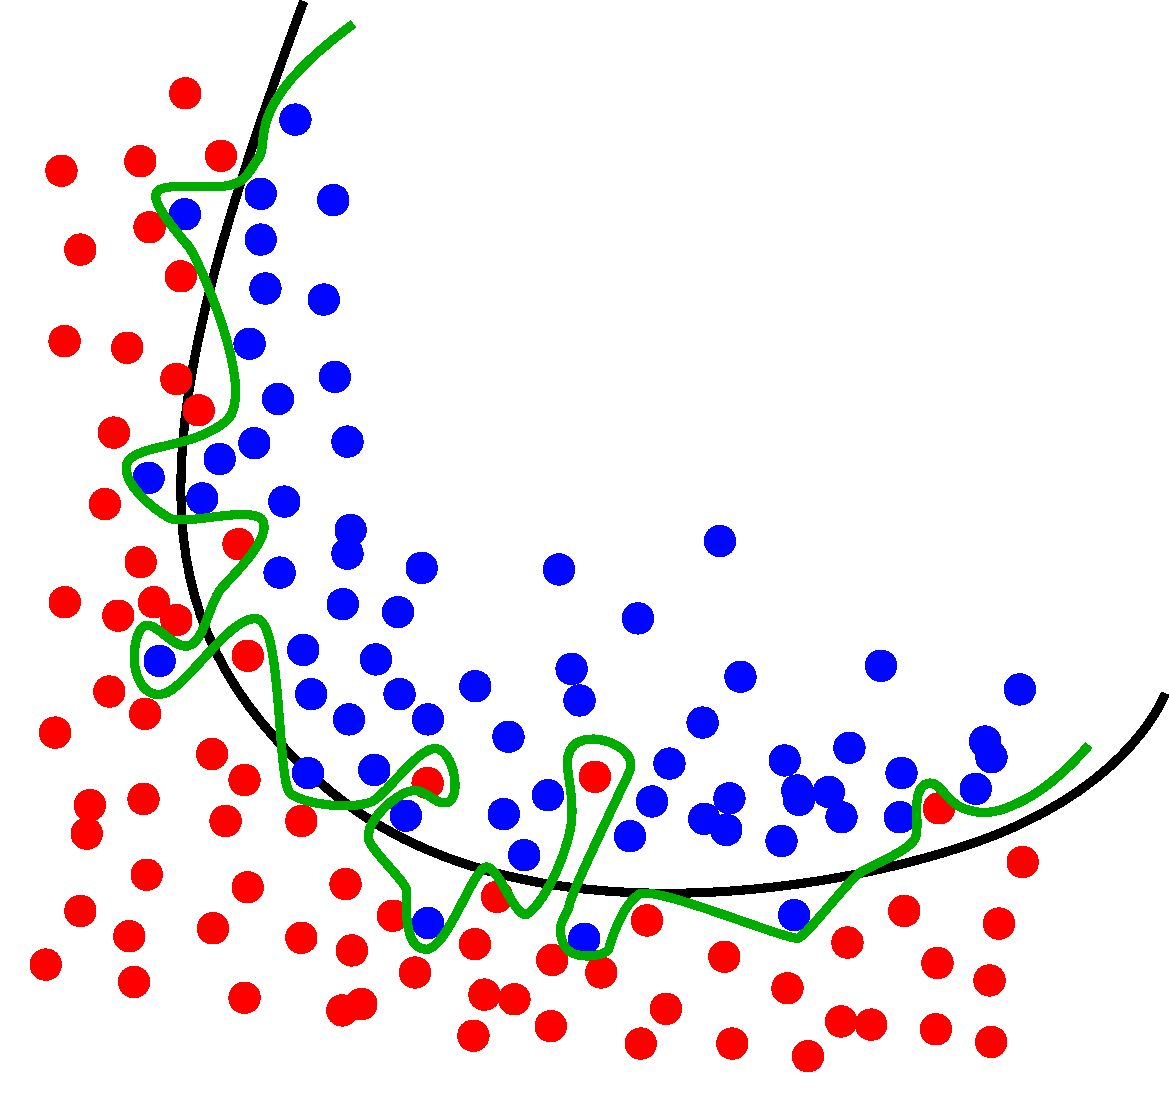
\includegraphics[width=0.45\textwidth]{Figures/implementation/overfitting.pdf}
	\caption{Příklad overfittingu. Černě je znázorněna kýžená funkce, zatímco červeně je vyznačena výsledná funkce, která je ovlivněná šumem v trénovací množině. (převzato z \cite{wiki_overfitting})}
	\label{fig:overfitting}
\end{figure}

Třída \texttt{SequentialDataset} provádí augmentaci dat celkem třemi způsoby.
\begin{description}
\item[horizontální převrácení] Při každém dotazu na získání prvku trénovací množiny je padesátiprocentní šance, že snímky výsledné množiny a související základní pravda budou horizontálně převráceny.

\item[náhodné škálování]
Pokud dataset obsahuje například snímky lidí jdoucích po chodníku, který je kolmý ke směru pohledu kamery, budou mít jednotliví lidé v obraze zhruba stejnou velikost hlav.
Přiblížením či oddálením se zároveň zvětší či zmenší velikost objektů v obrazech, důsledkem čehož bude mnohem větší rozmanitost datasetu.
Natrénovaný model tak bude mnohem robustnější vůči rozdílným velikostem hlav v obraze způsobených perspektivou.

\item[náhodné ořezání]
Jak bylo zmíněno v kapitole \ref{sec:Datasets}, řada datasetů obsahuje snímky ve vysokém rozlišení.
Toho může být využito pro augmentaci dat tak, že pokaždé, když má být snímek použit, je z něj vyřezána jiná část, která je následně předána neuronové síti.
Jelikož mají tyto snímky stovky tisíc pixelů, bude i ořezaný obrázek v dostatečně dobré kvalitě a neuronová síť tak může mít na vstupu mnohem větší množství rozdílných snímků.


\end{description}

K ořezání snímku by stejně muselo dojít, jelikož velikost vstupních snímků musí být kvůli skrytým stavům ConvLSTM známa předem a v datasetech se mohou nacházet sekvence snímků o různých velikostech a poměrech stran. Škálování obrazů na jednotnou velikost by v takovém případě mělo za výsledek deformaci snímků.
Při trénování tak síť na vstupu očekává obrazy o velikosti 512*512 pixelů.
Jelikož síť tvoří pouze konvoluční vrstvy a výstup konvoluční sítě nesměřuje do žádné plně propojené vrstvy, počet vah v síti se nemění a při nasazení modelu na reálných datech může být síť instancována pro jakkoliv velké obrazy.

\section{Neuronová síť}
Implementace samotné neuronové sítě je díky použití frameworku PyTorch velmi prostá.
Například jsou v tomto frameworku již dostupné implementace mnoha variant sítě ResNet, tudíž tato síť nemusí být implementována od základu.
V této práci proto byla použita dostupná síť ResNet-18.
Tato implementace je původně přizpůsobená pro dataset ImageNet, což je rozsáhlý dastaset určený pro klasifikaci objektů v obraze.
Celkem obsahuje více než 20 000 různých tříd objektů a síť dostupná ve frameworku Pytorch je proto zakončena plně propojenou (fully connected) částí, která obsahuje stejné množství výstupních neuronů.
Tato část byla ze sítě sítě odstraněna, aby výstupem sítě ResNet-18 nebyl vektor, nýbrž třídimenzionální tenzor, se kterým mohou dále pracovat další konvoluční vrstvy.
V implementované síti byla použita předtrénovaná verze sítě ResNet-18, což znamená že její váhy byly předtím nastaveny trénováním na datasetu ImageNet \cite{imagenet}, s cílem využít možnost, že nízkoúrovňové příznaky, které jsou extrahovány při klasifikaci objektů by se mohly podobat příznakům extrahovaným při vytváření hustotní mapy a využít tak efektu přenosového učení (Transfer learning) a urychlit tak nastavení správných hodnot vah v síti.

Implementace ConvLSTM je založená na projektu ConvLSTM-Pytorch dostupného z \cite{convlstm_pytorch}, jenž implementuje ConvLSTM síť pomocí frameworku PyTorch a aplikuje ji na problém MovingMNIST \cite{moving_mnist}.

ConvLSTM vrstva potřebuje při vytváření sítě znát velikost vstupního tenzoru (výška, šířka, počet kanálů, délka vstupní sekvence), velikost konvolučního filtru a počet kanálů v tenzoru výstupním.
Podle těchto informací mohou být vytvořeny skryté stavy, které mají stejnou šířku a výšku jako vstupní tenzor a jejich počet kanálů je stejný jako v tenzoru výstupním.
Tyto stavy jsou při zpracovávání prvního snímku frekvence nastaveny na nulové hodnoty.

Při dopředném šíření signálu ComvLSTM buňkou dojde ke konkatenaci vstupního tenzoru se skrytým stavem buňky a takto získaný tenzor je dán na vstup konvolučních filtrů, jejichž počet je roven čtyřnásobku počtu kanálů ve výstupním tenzoru, což je dáno tím, že s tímto tenzorem pracují c ConvLSTM buňce celkem čtyři brány.
Po aplikování konvolucí je výsledek rozdělen na čtyři části a každá z těchto částí je dána na vstup patřičné brány.
Následně na základě výstupu těchto bran je vypočítán nový stav buňky a z něj nový stav skrytého stavu a výstup.

\begin{lstlisting}[language=Python, caption={kód popisující dopředné šíření signálu v ConvLSTM vrstvě}]    
# sloučení vstupu a skrytého stavu a aplikování konvoluce
combined = torch.cat((x, hx), 1)
gates = self.conv(combined) 

# rozdělení na 4 části
ingate, forgetgate, cellgate, outgate = torch.split(
													gates,
													self.num_features,
													dim=1)
# aplikování bran ConvLSTM buňky
ingate = torch.sigmoid(ingate)		# vstupní brána
forgetgate = torch.sigmoid(forgetgate)	# zapomínací brána
cellgate = torch.tanh(cellgate)	# vstupní modulační brána
outgate = torch.sigmoid(outgate) # výstupní brána

# výpočet nového stavu buňky a skrytého stavu
cy = (forgetgate * cx) + (ingate * cellgate)
hy = outgate * torch.tanh(cy)
output_inner.append(hy)
hx = hy
cx = cy
\end{lstlisting}

Celou ConvLSTM část sítě zastřešuje třída \texttt{Encoder}.
Ta počítá s tím, že mezi jednotlivými ConvLSTM vrstvami se mohou nacházet vrstvy jiného typu.
Při vytváření této třídy jsou proto vyžadovány dva seznamy stejné velikosti.
Jeden z nich obsahuje seznam ConvLSTM vrstev s nastavenými parametry a druhý obsahuje seznamy konvolučních, dekonvolučních a poolingových vrstev, kterými signál prochází bezprostředně před zpracováním ConvLSTM vrstvou.
V případě, že nerekurentní složka v síti není potřeba, může být na vstupu pouze prázdný seznam.
Při dopředném šíření signálu pracuje na etapy, kdy každá etapa začínám aplikováním odpovídající nerekurentní sítě ze seznamu na vstupní data a následně předání sekvence zpracovaných dat na vstup ConvLSTM vrstvy.
Sekvence výstupů ConvLSTM vrstvy je následně dána na vstup následující etapy.

V navržené síti byly použity dvě ConvLSTM vrstvy, s tím, že před aplikováním každé z nich byla na vstup aplikována konvoluce o velikosti 3x3 s Leaky ReLU (Leaky Rectified Linear Unit) \cite{LeakyReLU} aktivační funkcí.
První konvoluční vrstva sníží dimenzi výstupu ze sítě ResNet a z vektorů o 512 prvcích uložených v jednotlivých pixelech vytvoří vektory o délce 64. 
S takto velkými tenzory pracují i ConvLSTM vrstvy.
Jejich vstup tedy má stejnou výšku a šířku jako výstup sítě ResNet, avšak mají pouze 64 kanálů.

Výstup pro poslední prvek vstupní sekvence je dán na vstup poslední části sítě, jejímž účelem je vytvořit výslednou hustotní mapu.
Jelikož je ale po zpracování vstupního obrazu sítí ResNet a ConvLSTM částí sítí výška i šířka výsledného tenzoru poměrně malá, je nejdříve tento tenzor pomocí bilineární interpolace zvětšen na šestnáctinásobek své velikosti.
Takto zvětšený tenzor je zpracován dvěma konvolučními vrstvami o velikosti 3x3 a následně je předložen konvoluci o velikosti 1, která vytvoří jednokanálový obraz, který je výslednou hustotní mapou.

\section{Trénování}
O trénování modelu se stará třída Trainer, jejíž implementace je založena na implementaci k článku \cite{DM_Count}.
Ta na základě vstupních parametrů instancuje třídu trénovacího datasetu a trénovanou neuronovou síť.
Síť je trénovaná po epochách, kde celkový počet epoch je stanovený parametrem, který zadá uživatel.
V každé epoše se postupně projdou všechny sekvence snímků obsažené v trénovací množině, pro každou sekvenci se vypočítá chyba, která je následně zpětně šířená sítí a základě které následně dochází k změně vah v síti.
Uživatel má možnost před spuštěním trénování nastavit parametry udávající váhu vlivu účelových funkcí OT Loss a TV Loss, celkový počet epoch, po které se bude estimátor trénovat, rychlost učení (learning rate), či délku sekvencí získaných z trénovací množiny, pomocí kterých se bude neuronová síť učit, a krok mezi jednotlivými snímky v této sekvenci.

\begin{figure}[h!]
	\centering
	% GNUPLOT: LaTeX picture with Postscript
\begingroup
  \makeatletter
  \providecommand\color[2][]{%
    \GenericError{(gnuplot) \space\space\space\@spaces}{%
      Package color not loaded in conjunction with
      terminal option `colourtext'%
    }{See the gnuplot documentation for explanation.%
    }{Either use 'blacktext' in gnuplot or load the package
      color.sty in LaTeX.}%
    \renewcommand\color[2][]{}%
  }%
  \providecommand\includegraphics[2][]{%
    \GenericError{(gnuplot) \space\space\space\@spaces}{%
      Package graphicx or graphics not loaded%
    }{See the gnuplot documentation for explanation.%
    }{The gnuplot epslatex terminal needs graphicx.sty or graphics.sty.}%
    \renewcommand\includegraphics[2][]{}%
  }%
  \providecommand\rotatebox[2]{#2}%
  \@ifundefined{ifGPcolor}{%
    \newif\ifGPcolor
    \GPcolortrue
  }{}%
  \@ifundefined{ifGPblacktext}{%
    \newif\ifGPblacktext
    \GPblacktexttrue
  }{}%
  % define a \g@addto@macro without @ in the name:
  \let\gplgaddtomacro\g@addto@macro
  % define empty templates for all commands taking text:
  \gdef\gplbacktext{}%
  \gdef\gplfronttext{}%
  \makeatother
  \ifGPblacktext
    % no textcolor at all
    \def\colorrgb#1{}%
    \def\colorgray#1{}%
  \else
    % gray or color?
    \ifGPcolor
      \def\colorrgb#1{\color[rgb]{#1}}%
      \def\colorgray#1{\color[gray]{#1}}%
      \expandafter\def\csname LTw\endcsname{\color{white}}%
      \expandafter\def\csname LTb\endcsname{\color{black}}%
      \expandafter\def\csname LTa\endcsname{\color{black}}%
      \expandafter\def\csname LT0\endcsname{\color[rgb]{1,0,0}}%
      \expandafter\def\csname LT1\endcsname{\color[rgb]{0,1,0}}%
      \expandafter\def\csname LT2\endcsname{\color[rgb]{0,0,1}}%
      \expandafter\def\csname LT3\endcsname{\color[rgb]{1,0,1}}%
      \expandafter\def\csname LT4\endcsname{\color[rgb]{0,1,1}}%
      \expandafter\def\csname LT5\endcsname{\color[rgb]{1,1,0}}%
      \expandafter\def\csname LT6\endcsname{\color[rgb]{0,0,0}}%
      \expandafter\def\csname LT7\endcsname{\color[rgb]{1,0.3,0}}%
      \expandafter\def\csname LT8\endcsname{\color[rgb]{0.5,0.5,0.5}}%
    \else
      % gray
      \def\colorrgb#1{\color{black}}%
      \def\colorgray#1{\color[gray]{#1}}%
      \expandafter\def\csname LTw\endcsname{\color{white}}%
      \expandafter\def\csname LTb\endcsname{\color{black}}%
      \expandafter\def\csname LTa\endcsname{\color{black}}%
      \expandafter\def\csname LT0\endcsname{\color{black}}%
      \expandafter\def\csname LT1\endcsname{\color{black}}%
      \expandafter\def\csname LT2\endcsname{\color{black}}%
      \expandafter\def\csname LT3\endcsname{\color{black}}%
      \expandafter\def\csname LT4\endcsname{\color{black}}%
      \expandafter\def\csname LT5\endcsname{\color{black}}%
      \expandafter\def\csname LT6\endcsname{\color{black}}%
      \expandafter\def\csname LT7\endcsname{\color{black}}%
      \expandafter\def\csname LT8\endcsname{\color{black}}%
    \fi
  \fi
    \setlength{\unitlength}{0.0500bp}%
    \ifx\gptboxheight\undefined%
      \newlength{\gptboxheight}%
      \newlength{\gptboxwidth}%
      \newsavebox{\gptboxtext}%
    \fi%
    \setlength{\fboxrule}{0.5pt}%
    \setlength{\fboxsep}{1pt}%
\begin{picture}(7200.00,4320.00)%
    \gplgaddtomacro\gplbacktext{%
      \colorrgb{0.00,0.00,0.00}%%
      \put(708,652){\makebox(0,0)[r]{\strut{}$0$}}%
      \colorrgb{0.00,0.00,0.00}%%
      \put(708,1031){\makebox(0,0)[r]{\strut{}$0.5$}}%
      \colorrgb{0.00,0.00,0.00}%%
      \put(708,1411){\makebox(0,0)[r]{\strut{}$1$}}%
      \colorrgb{0.00,0.00,0.00}%%
      \put(708,1790){\makebox(0,0)[r]{\strut{}$1.5$}}%
      \colorrgb{0.00,0.00,0.00}%%
      \put(708,2170){\makebox(0,0)[r]{\strut{}$2$}}%
      \colorrgb{0.00,0.00,0.00}%%
      \put(708,2549){\makebox(0,0)[r]{\strut{}$2.5$}}%
      \colorrgb{0.00,0.00,0.00}%%
      \put(708,2928){\makebox(0,0)[r]{\strut{}$3$}}%
      \colorrgb{0.00,0.00,0.00}%%
      \put(708,3308){\makebox(0,0)[r]{\strut{}$3.5$}}%
      \colorrgb{0.00,0.00,0.00}%%
      \put(708,3687){\makebox(0,0)[r]{\strut{}$4$}}%
      \colorrgb{0.00,0.00,0.00}%%
      \put(820,448){\makebox(0,0){\strut{}$0$}}%
      \colorrgb{0.00,0.00,0.00}%%
      \put(1573,448){\makebox(0,0){\strut{}$5$}}%
      \colorrgb{0.00,0.00,0.00}%%
      \put(2326,448){\makebox(0,0){\strut{}$10$}}%
      \colorrgb{0.00,0.00,0.00}%%
      \put(3079,448){\makebox(0,0){\strut{}$15$}}%
      \colorrgb{0.00,0.00,0.00}%%
      \put(3832,448){\makebox(0,0){\strut{}$20$}}%
      \colorrgb{0.00,0.00,0.00}%%
      \put(4584,448){\makebox(0,0){\strut{}$25$}}%
      \colorrgb{0.00,0.00,0.00}%%
      \put(5337,448){\makebox(0,0){\strut{}$30$}}%
      \colorrgb{0.00,0.00,0.00}%%
      \put(6090,448){\makebox(0,0){\strut{}$35$}}%
      \colorrgb{0.00,0.00,0.00}%%
      \put(6843,448){\makebox(0,0){\strut{}$40$}}%
    }%
    \gplgaddtomacro\gplfronttext{%
      \csname LTb\endcsname%%
      \put(186,2169){\rotatebox{-270}{\makebox(0,0){\strut{}Chyba sítě}}}%
      \csname LTb\endcsname%%
      \put(3831,142){\makebox(0,0){\strut{}Epocha}}%
      \csname LTb\endcsname%%
      \put(5978,3504){\makebox(0,0)[r]{\strut{}chyba sítě navržené sítě}}%
      \csname LTb\endcsname%%
      \put(3831,3993){\makebox(0,0){\strut{}Pozorovaná chyba sítě při trénování s použitím sinkhornova algoritmu}}%
    }%
    \gplbacktext
    \put(0,0){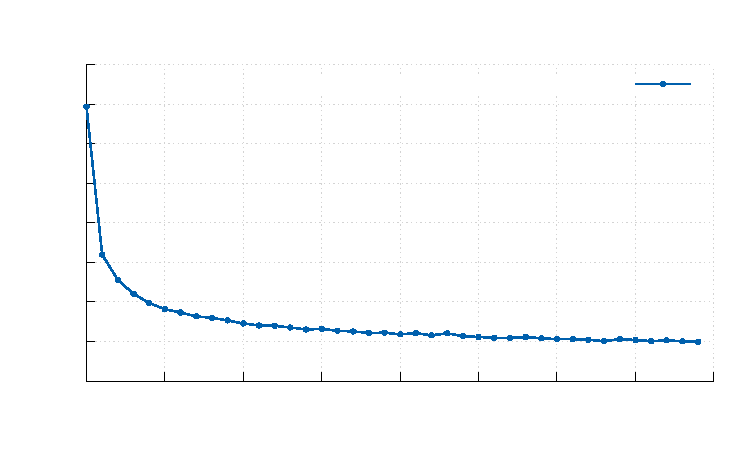
\includegraphics[width={360.00bp},height={216.00bp}]{Figures/solution/training_loss.pdf}}%
    \gplfronttext
  \end{picture}%
\endgroup

	\caption{Graf zobrazuje pozorovanou míru chyby při trénování navržené sítě.}
	\label{fig:loss_change}
\end{figure}

\endinput